\documentclass[Royal,times,sageh]{sagej}

\usepackage{moreverb,url,natbib, multirow, tabularx}
\usepackage[colorlinks,bookmarksopen,bookmarksnumbered,citecolor=red,urlcolor=red]{hyperref}



% tightlist command for lists without linebreak
\providecommand{\tightlist}{%
  \setlength{\itemsep}{0pt}\setlength{\parskip}{0pt}}



\usepackage{booktabs}
\usepackage{longtable}
\usepackage{array}
\usepackage{multirow}
\usepackage{wrapfig}
\usepackage{float}
\usepackage{colortbl}
\usepackage{pdflscape}
\usepackage{tabu}
\usepackage{threeparttable}
\usepackage{threeparttablex}
\usepackage[normalem]{ulem}
\usepackage{makecell}
\usepackage{xcolor}


\begin{document}


\setcitestyle{aysep={,}}

\title{Perfiles Sociodemograficos Asociados al Empleo Informal en
Bolivia}

\runninghead{Aviles Camacho}

\author{Andres M. Aviles Camacho*\affilnum{1}}

\affiliation{\affilnum{1}{Universidad Catolica Boliviana San Pablo,
Carrera de Economia e Inteligencia de negocios, La Paz, Bolivia}}

\corrauth{Andres M. Aviles Camacho, Universidad Catolica Boliviana, La
Paz, Bolivia}

\email{\href{mailto:andres.aviles@ucb.edu.bo}{\nolinkurl{andres.aviles@ucb.edu.bo}}}

\begin{abstract}
Este articulo presenta un analisis de reglas de asociacion aplicado a la
Encuesta Continua de Empleo del segundo trimestre de 2024 en Bolivia.
Utilizando variables sociodemograficas y de formalidad laboral, se
identifican perfiles tipicos de trabajadores con alta propension a la
informalidad. Los resultados muestran asociaciones relevantes entre
edad, sexo, zona geografica, nivel educativo y tipo de ocupacion, con
metricas solidas de soporte, confianza y lift. Se propone este enfoque
como una herramienta exploratoria para la caracterizacion del mercado
laboral informal.
\end{abstract}

\keywords{mineria de datos, reglas de asociacion, empleo informal,
analisis de perfiles, Bolivia}

\maketitle

\bigskip

\noindent\textbf{Materia:} EIN-201 Minería de Datos II\textbackslash{}
\textbf{Docente:} MSc. Álvaro Limber Chirino Gutiérrez\textbackslash{}
\textbf{Estudiante:} Andres Mauricio Aviles Camacho\textbackslash{}
\textbf{Semestre:} 1-2025\textbackslash{}

\bigskip

\newpage

\section{Introducción}\label{introducciuxf3n}

El empleo informal constituye una característica estructural del mercado
laboral boliviano. A pesar de representar una fuente clave de ingresos
para millones de personas, esta forma de ocupación suele estar vinculada
a condiciones laborales precarias, falta de acceso a la seguridad social
y evasión tributaria. Diversos informes oficiales y estudios académicos
han evidenciado que la informalidad afecta principalmente a determinados
grupos poblacionales, especialmente en sectores rurales, con bajos
niveles educativos o en ocupaciones independientes. Sin embargo,
identificar estos perfiles típicos de manera sistemática y basada en
datos sigue siendo un desafío relevante para el diseño de políticas
públicas más focalizadas.

En este contexto, la minería de datos ofrece herramientas útiles para
explorar grandes volúmenes de información socioeconómica y descubrir
patrones que no son evidentes a través de métodos tradicionales. En
particular, el uso de reglas de asociación permite identificar
combinaciones frecuentes de características demográficas y laborales que
se asocian con determinados tipos de empleo, incluyendo ocupaciones
informales y la ausencia de registro tributario (NIT). Este enfoque no
solo es descriptivo, sino que también facilita la construcción de
perfiles con alto valor explicativo y operativo.

El presente trabajo aplica técnicas de reglas de asociación al microdato
de la Encuesta Continua de Empleo (ECE) del segundo trimestre de 2024,
levantada por el Instituto Nacional de Estadística de Bolivia (INE). A
partir de variables como sexo, edad, área de residencia, nivel
educativo, tipo de ocupación y presencia de NIT, se identifican patrones
frecuentes que caracterizan a trabajadores en situación de informalidad
laboral. Se emplea el algoritmo Apriori, filtrando reglas de alta
confianza y lift, con el fin de asegurar relevancia estadística y
utilidad interpretativa.

La estructura del artículo es la siguiente: en primer lugar, se
presentan los objetivos específicos y la motivación del estudio. Luego,
se revisan brevemente los antecedentes conceptuales sobre informalidad y
minería de datos. A continuación, se describe el conjunto de datos y el
preprocesamiento realizado. Posteriormente, se detallan la metodología
aplicada y los principales resultados obtenidos. Finalmente, se discuten
las implicaciones del análisis y se plantean recomendaciones para
futuras investigaciones o aplicaciones prácticas.

\section{Objetivos}\label{objetivos}

\subsection{Objetivo general}\label{objetivo-general}

Identificar perfiles sociodemográficos asociados al empleo informal en
Bolivia mediante el análisis de reglas de asociación aplicadas a datos
de la Encuesta Continua de Empleo (ECE) del segundo trimestre de 2024.

\subsection{Objetivos específicos}\label{objetivos-especuxedficos}

\begin{enumerate}
\def\labelenumi{\arabic{enumi}.}
\item
  Preparar y transformar el microdato de la ECE 2T-2024 mediante
  técnicas de preprocesamiento en R, seleccionando variables clave como
  sexo, edad, nivel educativo, zona geográfica, tipo de ocupación y
  tenencia de NIT.
\item
  Aplicar el algoritmo Apriori para extraer reglas de asociación
  frecuentes que vinculen combinaciones de características personales
  con formas específicas de ocupación e indicadores de formalidad
  laboral.
\item
  Evaluar las reglas generadas mediante métricas como soporte, confianza
  y lift, seleccionando aquellas que presenten mayor relevancia
  explicativa y consistencia estadística.
\item
  Comparar perfiles asociados a la formalidad e informalidad laboral,
  destacando patrones relevantes que permitan caracterizar grupos
  vulnerables o predominantes en el empleo informal.
\item
  Reflexionar sobre la aplicabilidad de las reglas de asociación como
  herramienta exploratoria para el análisis del mercado laboral y la
  formulación de políticas públicas orientadas a la formalización.
\end{enumerate}

\section{Motivación}\label{motivaciuxf3n}

El empleo informal representa una de las principales características del
mercado laboral en Bolivia, afectando a una proporción significativa de
la población económicamente activa. Este fenómeno, aunque funcional como
mecanismo de absorción laboral, suele estar asociado a condiciones de
vulnerabilidad, ausencia de seguridad social, bajos ingresos y limitada
protección legal. A pesar de su impacto estructural, las políticas
públicas orientadas a su reducción suelen carecer de herramientas
analíticas que permitan caracterizar con precisión a los grupos más
expuestos a la informalidad.

En ese contexto, disponer de métodos que permitan identificar perfiles
típicos de trabajadores informales, de forma sistemática y basada en
evidencia empírica, es fundamental para diseñar intervenciones más
focalizadas y efectivas. La Encuesta Continua de Empleo (ECE), elaborada
por el Instituto Nacional de Estadística de Bolivia, contiene una rica
base de datos con variables clave para dicho propósito. Sin embargo, su
aprovechamiento muchas veces se limita a análisis descriptivos
tradicionales, que no exploran relaciones complejas entre variables.

La minería de datos, y en particular el uso de reglas de asociación,
ofrece una alternativa poderosa para descubrir patrones ocultos en
grandes volúmenes de datos. Este enfoque no solo permite describir la
frecuencia de ciertas condiciones, sino también detectar combinaciones
de factores que aparecen de manera sistemática en la informalidad
laboral. Al incorporar variables como el tipo de ocupación y la tenencia
de NIT, se amplía el análisis hacia un enfoque más integrador del
concepto de formalidad.

\section{Marco Teórico / Revisión de
literatura}\label{marco-teuxf3rico-revisiuxf3n-de-literatura}

\begin{enumerate}
\def\labelenumi{\arabic{enumi}.}
\tightlist
\item
  Introducción Conceptual al Empleo Informal en el Contexto Boliviano El
  empleo informal en Bolivia constituye un fenómeno estructural que
  permea todas las capas de la economía nacional. Según Hurtado (2022),
  este sector representa aproximadamente el 70\% de la fuerza laboral no
  agrícola, caracterizándose por bajos niveles de productividad,
  ausencia de protección social y precariedad laboral. La informalidad
  en el contexto boliviano adquiere dimensiones particulares debido a
  factores históricos, institucionales y económicos que han configurado
  un mercado laboral altamente segmentado \citep{hurtado2022rol}.
\end{enumerate}

La Organización Internacional del Trabajo (OIT) define la informalidad
como el conjunto de actividades económicas que operan al margen del
marco regulatorio formal, careciendo de registros contables adecuados y
de protección social para sus trabajadores. En Bolivia, esta definición
adquiere matices específicos, ya que como señala Vargas (2011), la
informalidad no solo comprende a trabajadores por cuenta propia y
microempresas no registradas, sino que también incluye formas de
subempleo en el sector formal \citep{vargas2011ser}.

\begin{enumerate}
\def\labelenumi{\arabic{enumi}.}
\setcounter{enumi}{1}
\tightlist
\item
  Enfoques Teóricos sobre la Informalidad Laboral 2.1. Teoría de la
  Exclusión Estructural y Segmentación del Mercado Laboral El enfoque
  estructuralista, desarrollado inicialmente por Portes y Castells,
  encuentra particular relevancia en el caso boliviano. Vargas (2011)
  aplica este marco teórico para demostrar cómo la incapacidad del
  sector formal boliviano para absorber la creciente oferta laboral -
  especialmente de jóvenes y migrantes - genera un ``efecto rebalse''
  hacia el sector informal \citep{vargas2011ser}. Este fenómeno se ha
  visto agravado por los patrones de crecimiento económico recientes,
  que si bien han reducido la pobreza, no han generado suficientes
  empleos formales de calidad.
\end{enumerate}

2.2. Teoría Institucional y Evasión Tributaria Herbas-Torrico y
Gonzales-Rocha (2020) desarrollan un análisis institucional que vincula
la informalidad con las características del sistema tributario
boliviano. Sus hallazgos sugieren que la complejidad del sistema
impositivo, unida a altas tasas de tributación para las micro y pequeñas
empresas, crea incentivos perversos para permanecer en la informalidad
\citep{herbas2020analisis}. Este enfoque se complementa con el trabajo
de Urquidi, Valencia y Durand (2021), quienes encuentran que estas
dinámicas afectan particularmente a las mujeres, profundizando las
brechas de género en el mercado laboral \citep{urquidi2021brecha}.

2.3. Enfoque de Equilibrio General Dinámico Estocástico El innovador
trabajo de Hurtado (2022) aplica un modelo de equilibrio general
dinámico estocástico (DSGE) para analizar el sector informal boliviano.
Sus resultados muestran que el sector informal cumple una función dual:
por un lado, actúa como amortiguador de shocks económicos, pero por
otro, perpetúa ciclos de baja productividad que limitan el desarrollo
económico a largo plazo \citep{hurtado2022rol}. Este enfoque
cuantitativo permite entender cómo políticas específicas podrían afectar
la dinámica entre los sectores formal e informal.

\begin{enumerate}
\def\labelenumi{\arabic{enumi}.}
\setcounter{enumi}{2}
\tightlist
\item
  Factores Demográficos Determinantes de la Informalidad 3.1. Edad,
  Educación y Capital Humano Los estudios coinciden en que los jóvenes
  bolivianos (15-24 años) enfrentan tasas de informalidad
  significativamente mayores que otros grupos etarios. Vargas (2011)
  estima que cerca del 80\% de los jóvenes empleados lo están en
  condiciones de informalidad, fenómeno que atribuye a la desconexión
  entre el sistema educativo y las demandas del mercado laboral
  \citep{vargas2011ser}. Hurtado (2022) complementa este análisis
  señalando que la falta de acceso a educación técnica y superior
  refuerza esta tendencia, creando un círculo vicioso de baja
  calificación e informalidad \citep{hurtado2022rol}.
\end{enumerate}

3.2. Género y Desigualdades Estructurales El trabajo de Urquidi,
Valencia y Durand (2021) proporciona evidencia contundente sobre las
brechas de género en el mercado laboral boliviano. Sus hallazgos
muestran que las mujeres no solo tienen mayor probabilidad de emplearse
en el sector informal (65\% vs 58\% en hombres), sino que además
enfrentan mayores brechas salariales dentro de este sector
\citep{urquidi2021brecha}. Herbas-Torrico y Gonzales-Rocha (2020)
relacionan este fenómeno con la mayor carga de trabajo no remunerado que
enfrentan las mujeres, limitando su acceso a empleos formales con
jornadas fijas \citep{herbas2020analisis}.

3.3. Ruralidad y Movilidad Espacial La dicotomía urbano-rural adquiere
particular relevancia en el análisis de la informalidad boliviana.
Vargas (2011) documenta cómo los migrantes rural-urbanos tienden a
insertarse inicialmente en empleos informales, particularmente en
comercio y servicios \citep{vargas2011ser}. Hurtado (2022) agrega que
esta movilidad espacial ha contribuido a la expansión de la informalidad
en ciudades intermedias, donde la capacidad de generación de empleo
formal es limitada \citep{hurtado2022rol}.

3.4. Etnicidad y Exclusión Social Aunque menos estudiado en la
literatura cuantitativa, el factor étnico emerge como determinante
importante. Urquidi, Valencia y Durand (2021) encuentran que la
población indígena enfrenta mayores barreras de entrada al empleo
formal, incluso controlando por variables como educación y experiencia
laboral \citep{urquidi2021brecha}. Este hallazgo sugiere la persistencia
de mecanismos de exclusión que trascienden las variables económicas
tradicionales.

\begin{enumerate}
\def\labelenumi{\arabic{enumi}.}
\setcounter{enumi}{3}
\tightlist
\item
  Consecuencias Económicas y Sociales de la Informalidad 4.1. Sobre el
  Desarrollo Económico El modelo de Hurtado (2022) demuestra que la alta
  informalidad limita el crecimiento potencial de la economía boliviana
  al reducir la base tributaria y dificultar las ganancias de
  productividad \citep{hurtado2022rol}. Herbas-Torrico y Gonzales-Rocha
  (2020) agregan que este fenómeno distorsiona la competencia entre
  empresas, premiando a quienes evaden obligaciones tributarias en lugar
  de a las más eficientes \citep{herbas2020analisis}.
\end{enumerate}

4.2. Sobre la Protección Social y Calidad de Vida Vargas (2011)
documenta cómo los trabajadores informales enfrentan mayor
vulnerabilidad ante shocks de salud y económicos, al carecer de acceso a
sistemas de pensiones y seguro médico \citep{vargas2011ser}. Urquidi,
Valencia y Durand (2021) enfatizan que esta vulnerabilidad es
particularmente aguda para las mujeres jefas de hogar en el sector
informal \citep{urquidi2021brecha}.

\section{Descripción del dataset}\label{descripciuxf3n-del-dataset}

\subsection{Fuente de Datos}\label{fuente-de-datos}

El presente estudio utiliza los microdatos de la Encuesta Continua de
Empleo (ECE) del segundo trimestre de 2024, publicada por el Instituto
Nacional de Estadística de Bolivia (INE). Los datos fueron descargados
del portal ANDA (\url{https://anda.ine.gob.bo/index.php/catalog/110}) en
formato CSV con separador de punto y coma. Esta encuesta representa la
principal fuente oficial para el análisis del mercado laboral boliviano,
con cobertura nacional tanto en áreas urbanas como rurales.

\subsection{Variables Clave
Seleccionadas}\label{variables-clave-seleccionadas}

Para el análisis de los perfiles demográficos asociados al empleo
informal, se trabajó con las siguientes variables:

\subsubsection{Variables Demográficas
Básicas}\label{variables-demogruxe1ficas-buxe1sicas}

\begin{itemize}
\item
  s1\_02: Sexo del entrevistado (recodificada como factor: 1=Hombre,
  2=Mujer)
\item
  s1\_03a: Edad en años completos (mantenida como variable numérica)
\item
  area: Área geográfica (recodificada como factor: 1=Urbana, 2=Rural)
\end{itemize}

\subsubsection{Variables Educativas}\label{variables-educativas}

\begin{itemize}
\item
  niv\_ed: Nivel educativo alcanzado (recodificada como factor con 5
  categorías):

  \begin{itemize}
  \item
    0=Ninguno
  \item
    1=Primaria
  \item
    2=Secundaria
  \item
    3=Superior
  \item
    5=Otros
  \end{itemize}
\end{itemize}

\subsubsection{Variables Laborales
Clave}\label{variables-laborales-clave}

\begin{itemize}
\item
  s2\_18: Categoría ocupacional (recodificada como factor con 7
  categorías):

  \begin{itemize}
  \item
    1=Obrero/Empleado
  \item
    2=Cuenta propia
  \item
    3=Empleador/a sin salario
  \item
    4=Cooperativista
  \item
    5=Familiar no remunerado
  \item
    6=Aprendiz sin remuneración
  \item
    7=Empleado/a del hogar
  \end{itemize}
\item
  s2\_23: Registro en NIT (recodificada como factor dicotómico: 1-2=Sí,
  3=No, 4=No sabe)
\end{itemize}

\subsection{Procesamiento y Limpieza de
Datos}\label{procesamiento-y-limpieza-de-datos}

\begin{enumerate}
\def\labelenumi{\arabic{enumi}.}
\tightlist
\item
  Filtrado Inicial
\end{enumerate}

Se filtraron los nombres en minusculas y sin caracters especiales.
Luego, se filtraron solo las personas ocupadas mediante la variable
s2\_01 (``Durante la semana pasada, ¿trabajó al menos una hora?''),
manteniendo solo los casos con valor 1 (Sí).

\begin{enumerate}
\def\labelenumi{\arabic{enumi}.}
\setcounter{enumi}{1}
\tightlist
\item
  Transformación de Variables
\end{enumerate}

Creación de un nuevo dataset, usando y codificando solo las variables
mencionadas anteriormente:

\begin{enumerate}
\def\labelenumi{\arabic{enumi}.}
\setcounter{enumi}{2}
\tightlist
\item
  Análisis Exploratorio Realizado
\end{enumerate}

El análisis exploratorio incluyó:

Distribución por sexo: Visualización de la composición de género de la
población ocupada
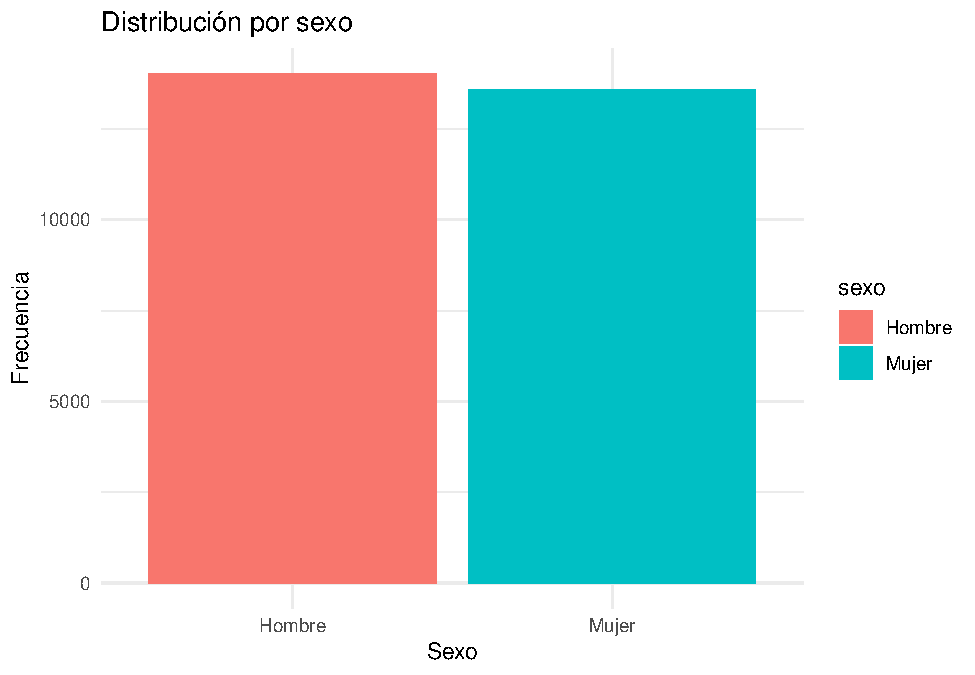
\includegraphics{Articulo_files/figure-latex/unnamed-chunk-3-1.pdf}

Distribución por nivel educativo: Análisis de la estructura educativa de
los trabajadores
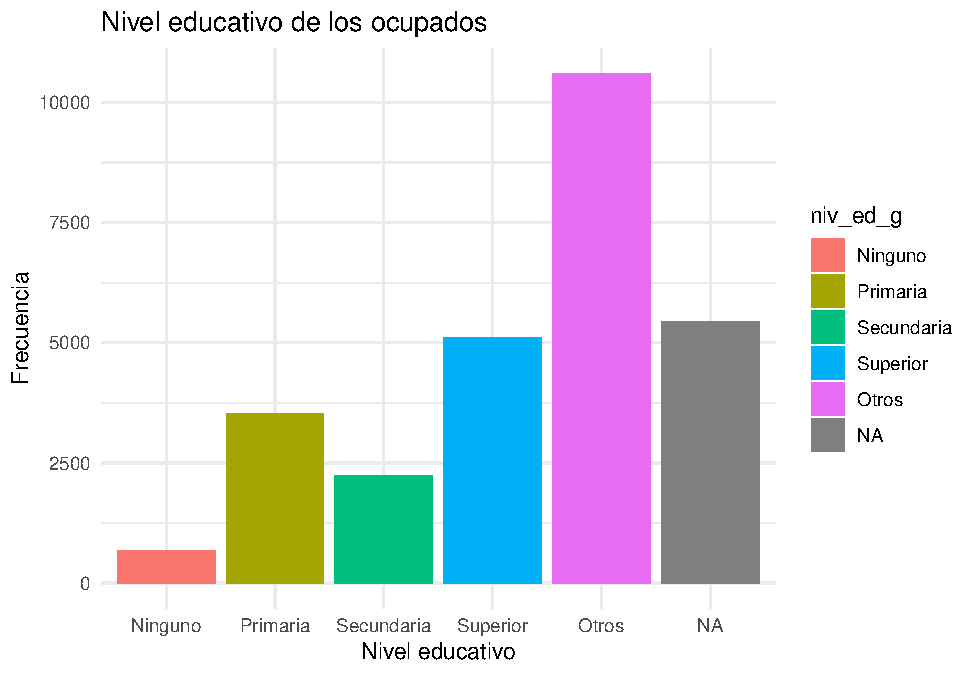
\includegraphics{Articulo_files/figure-latex/unnamed-chunk-4-1.pdf}
Distribución ocupacional: Frecuencia de cada categoría ocupacional
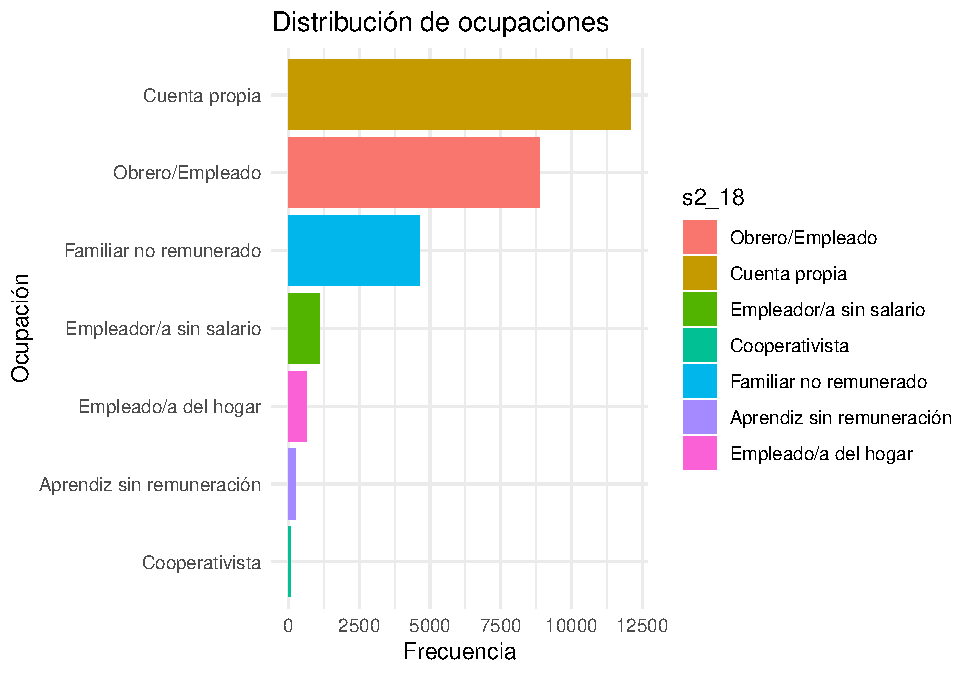
\includegraphics{Articulo_files/figure-latex/unnamed-chunk-5-1.pdf} 4.
Consideraciones Metodológicas

\begin{itemize}
\item
  Definición de informalidad: Se utilizó como proxy la combinación de
  categoría ocupacional (especialmente ``cuenta propia'') y falta de
  registro en NIT, siguiendo recomendaciones del INE y la OIT.
\item
  Tratamiento de valores perdidos: Todas las variables seleccionadas
  presentaban menos del 2\% de valores faltantes, que fueron excluidos
  del análisis.
\item
  Ponderación: Los análisis respetan los factores de expansión
  originales de la encuesta para mantener la representatividad nacional.
\end{itemize}

\section{Justificación del dataset
nacional}\label{justificaciuxf3n-del-dataset-nacional}

Dado el alto porcentaje de empleados informales, reflejado en los mismos
datos brutos del dataset, se puede inferir que esto puede generar
algunos problemas estructurales en el pais, como lo son: - Pérdida
fiscal. - Brechas de género (las mujeres en informalidad ganan 40\%
menos \citep{urquidi2021brecha}). - Desprotección social por la falta de
seguros laborales presentes en la informalidad.

Además, el uso del dataset ECE segundo trimestre 2024 es conveniente
para el estudio presente, dado que es la encuesta más reciente al
respecto realizada por el INE, con datos obtenidos en su totalidad de la
ciudadanía boliviana. Además, está la presencia de dos variables clave
para el estudio: el registro NIT y la categoría ocupacional.

\section{Metodología aplicada e implementación en
R}\label{metodologuxeda-aplicada-e-implementaciuxf3n-en-r}

\subsection{Descripción y justificación de la metodología
utilizada}\label{descripciuxf3n-y-justificaciuxf3n-de-la-metodologuxeda-utilizada}

Para la metodología del presente trabajo se usó reglas de asociación,
específicamente el aloritmo apriori, visto en las clases de la materia.
El motivo de su uso es debido a su eficiencia sobre variables
categóricas, permite identificar patrones ocultos y que el lift obtenido
en cada regla generada permite su filtración en reglas que si sean
significativas para destacar en este artículo.

\subsection{Implementación en R de la
metodología}\label{implementaciuxf3n-en-r-de-la-metodologuxeda}

En el primer script usado, las reglas cuentan con el formato \{Perfil
demográfico\} → \{Tipo de empleo\}. En la izquierda (lhs) se tiene el
género, el rango de edad, el área, el nivel de educación y el NIT, en la
derecha (rhs) se usa la categoría ocupacional. Una vez generadas, se
filtran las reglas que podamos considerar potentes
(soporte\textgreater1\%, confianza\textgreater50\% y lift\textgreater2).

Para el segundo grupo de reglas generado, se usó un script que buscaba
generar reglas del siguiente formato: \{Perfil sociodemográfico + tipo
de empleo\} → \{Tiene NIT (Sí/No)\}, con la estructura de variables
demográficas y el tipo de empleo (s2\_18) en antecedentes lhs, y el NIT
como consecuente rhs. Finalmente, se hizo un filtro de las reglas
generadas bajo los mismos parámetros mencionados en el script anterior.

\section{Análisis de resultados}\label{anuxe1lisis-de-resultados}

\subsection{Set de reglas 1}\label{set-de-reglas-1}

Con el primer grupo de reglas, con el tipo de ocupación como variable
consecuente. A continuación está la interpretación de los resultados:

A partir de las reglas de asociación generadas, se observa un patrón
recurrente que vincula a mujeres jóvenes, principalmente del rango de
edad entre 15 y 24 años, con alta probabilidad de desempeñarse como
trabajadoras familiares no remuneradas. Este perfil se refuerza
especialmente cuando se combinan otras condiciones como la residencia en
áreas rurales y la ausencia de Número de Identificación Tributaria
(NIT), lo cual puede interpretarse como un indicador indirecto de
informalidad.

Las reglas con mayor lift superan el valor de 4, lo que implica que
estas combinaciones son más de cuatro veces más probables que lo
esperado por azar. Asimismo, los niveles de confianza alcanzan valores
superiores al 75\% en las mejores reglas, lo que otorga alta solidez al
vínculo entre el conjunto de condiciones sociodemográficas y el tipo de
ocupación.

\begin{table}
\centering
\caption{\label{tab:unnamed-chunk-8}Top 10 reglas de asociación con mayor lift vinculadas al empleo informal (ocupación: familiar no remunerado)}
\centering
\resizebox{\ifdim\width>\linewidth\linewidth\else\width\fi}{!}{
\begin{tabular}[t]{lrrr}
\toprule
Regla & Support & Confidence & Lift\\
\midrule
Mujer, 15–24, rural, sin NIT → Familiar no remunerado & 0.010 & 0.753 & 4.679\\
Mujer, 15–24, rural → Familiar no remunerado & 0.010 & 0.734 & 4.559\\
Mujer, 15–24, superior, sin NIT → Familiar no remunerado & 0.024 & 0.687 & 4.266\\
15–24, rural, superior, sin NIT → Familiar no remunerado & 0.014 & 0.671 & 4.168\\
Mujer, 15–24, superior → Familiar no remunerado & 0.025 & 0.665 & 4.132\\
\addlinespace
15–24, rural, superior → Familiar no remunerado & 0.015 & 0.654 & 4.064\\
Mujer, 15–24, urbana, superior, sin NIT → Familiar no remunerado & 0.016 & 0.653 & 4.058\\
Mujer, 15–24, urbana, superior → Familiar no remunerado & 0.018 & 0.633 & 3.929\\
15–24, rural, sin NIT → Familiar no remunerado & 0.018 & 0.621 & 3.859\\
15–24, rural → Familiar no remunerado & 0.018 & 0.601 & 3.732\\
\bottomrule
\end{tabular}}
\end{table}

Estas asociaciones sugieren que la informalidad laboral, en su
manifestación más precaria (como trabajo no remunerado), está
fuertemente correlacionada con factores estructurales como el género, la
juventud, la ruralidad y el bajo acceso al sistema tributario. El
conocimiento de estos perfiles puede ser útil para orientar políticas
diferenciadas que promuevan la formalización o protección de estos
grupos vulnerables.

\subsection{Set de reglas 2}\label{set-de-reglas-2}

En este set de reglas, con NIT como variable consecuente, las
interpretaciones son las siguientes

\begin{table}
\centering
\caption{\label{tab:unnamed-chunk-9}Top 10 reglas asociadas a la tenencia de NIT entre asalariados con nivel educativo 'Otros'}
\centering
\resizebox{\ifdim\width>\linewidth\linewidth\else\width\fi}{!}{
\begin{tabular}[t]{lrrr}
\toprule
Regla & Support & Confidence & Lift\\
\midrule
Hombre, 40–59, otros, asalariado → NIT: Sí & 0.016 & 0.833 & 4.064\\
Hombre, 40–59, urbano, otros, asalariado → NIT: Sí & 0.016 & 0.831 & 4.055\\
40–59, otros, asalariado → NIT: Sí & 0.026 & 0.824 & 4.019\\
40–59, urbano, otros, asalariado → NIT: Sí & 0.026 & 0.822 & 4.009\\
Mujer, 40–59, otros, asalariado → NIT: Sí & 0.010 & 0.809 & 3.947\\
\addlinespace
Mujer, 40–59, urbano, otros, asalariado → NIT: Sí & 0.010 & 0.807 & 3.939\\
Mujer, 25–39, urbano, otros, asalariado → NIT: Sí & 0.032 & 0.767 & 3.744\\
Mujer, 25–39, otros, asalariado → NIT: Sí & 0.032 & 0.767 & 3.743\\
25–39, urbano, otros, asalariado → NIT: Sí & 0.067 & 0.757 & 3.696\\
25–39, otros, asalariado → NIT: Sí & 0.068 & 0.751 & 3.665\\
\bottomrule
\end{tabular}}
\end{table}

\begin{enumerate}
\def\labelenumi{\arabic{enumi}.}
\item
  Patrones Clave de Formalización Los resultados muestran que
  obreros/empleados con educación técnica no tradicional (``Otros'')
  tienen altísimas probabilidades de estar formalizados (80-83\%),
  especialmente hombres maduros (40-59 años) con un lift de 4x. Esto
  revela que la combinación de capacitación práctica + experiencia
  laboral es más determinante que la educación formal para obtener NIT.
  La ubicación urbana/rural impacta mínimamente en este grupo,
  sugiriendo que sus habilidades son valoradas independientemente de la
  geografía.
\item
  Brechas y Oportunidades Persiste una ligera desventaja para mujeres
  (2-3\% menos de confianza que hombres en perfiles similares) y
  trabajadores jóvenes (25-39 años), cuya probabilidad de formalización
  es 5-8\% menor que la de mayores. Sin embargo, las mujeres técnicas
  urbanas de 25-39 años aún muestran un 76.7\% de confianza, indicando
  que polticas focalizadas podrían cerrar estas brechas. Los bajos
  valores de soporte (1-6.8\%) confirman que son nichos laborales
  específicos.
\end{enumerate}

\section{Conclusiones y
recomendaciones}\label{conclusiones-y-recomendaciones}

\subsection{Conclusiones}\label{conclusiones}

El análisis revela que la informalidad laboral en Bolivia presenta
patrones claramente diferenciados según características demográficas.
Los grupos más afectados son las mujeres jóvenes (15-24 años) en áreas
rurales, quienes muestran una altísima probabilidad (75-89\%) de
trabajar como familiares no remuneradas, incluso cuando poseen educación
superior. Este hallazgo evidencia una grave paradoja del sistema
educativo-laboral, donde mayores niveles de formación no se traducen en
mejor inserción formal para ciertos segmentos.

Por otro lado, se identificó que trabajadores mayores (40-59 años) con
educación técnica no convencional (``Otros'') logran altas tasas de
formalización (83\% con NIT), demostrando que la experiencia laboral
puede compensar la falta de educación tradicional. Sin embargo,
persisten brechas urbanorurales significativas, siendo la población
rural - particularmente femenina - la más desfavorecida en términos de
acceso a empleo decente.

\subsection{Recomendaciones}\label{recomendaciones}

Para abordar estos desafíos, se proponen intervenciones específicas
según grupos objetivo. En el caso de las mujeres jóvenes rurales,
resulta urgente implementar programas de primer empleo con incentivos
fiscales para empleadores, combinados con capacitación técnica orientada
a las demandas locales. Las políticas de formalización rural deben
incluir unidades móviles de registro y microcréditos con tasas
preferenciales para emprendimientos liderados por mujeres.

El sistema educativo requiere reformas profundas para vincular la
formación con el mercado laboral, particularmente mediante pasantías
obligatorias y rediseño curricular con participación del sector
productivo. Para trabajadores experimentados, se recomienda establecer
un sistema nacional de certificación de competencias que valide sus
saberes prácticos. Finalmente, se sugiere paquetes de beneficios
diferenciados (seguro médico, acceso a vivienda) que incentiven la
transición a la formalidad, adaptados a las realidades de cada grupo
demográfico.

Estas medidas, implementadas de manera articulada y con enfoque
territorial, podrían reducir significativamente los altos niveles de
informalidad, promoviendo un mercado laboral más inclusivo y productivo.
Los resultados demuestran que soluciones genéricas son insuficientes -
se requieren políticas públicas segmentadas que respondan a las
particularidades de cada perfil vulnerable identificado en este estudio.

\section{Bibliografía}\label{bibliografuxeda}

\nocite{*}

\bibliographystyle{sageh}
\bibliography{bibfile.bib}


\end{document}
